\subsection{Runtime} 
\label{sec:runtime}
In the sleep phase, we trained the variational approximation on 
$100 \times 100$ images. Note however, our variational posterior can be evaluated on images of arbitrary size, by tiling the image into $s \times s$ tiles. On the crowded starfield described below, we used $s = 2$. 

We trained the initial sleep phase with the PSF and background set to SDSS estimates. We trained for 200 epochs with 200 images per epoch. We used 
the Adam optimization routine~\cite{kingma2014adam} set at its default parameters. On a single GPU (TODO: give some specs?), this initial sleep phase took approximately 10 minutes. 

We ran two further wake-sleep cycles with each cycle taking approximately a minute. 

After training, evaluating the approximate posterior on a $100 \times 100$ 
image took $\approx 0.2$ seconds. By comparison, PCAT, which runs MCMC, 
reported a runtime of 30 minutes. 

We emphasize that our speed at inference time is what enables our method to 
scale up to large astronomical surveys. An SDSS image is $1489 \times 2048$ 
pixels. Thus, PCAT would require 
$\approx 30\text{min} \times 14 \times 20 = 8400$min, or almost six days to run.\footnote{TODO: 
Maybe this isn't quite fair? I suspect MCMC will scale
with the number of stars, not the size of an image. I think we can make 
this more precise.}
In contrast, if we assume the PSF and background are relatively homogeneous 
across the full SDSS image (which PCAT also assumes), we can 
train our variational approximation on a small $100 \times 100$ subimage
(while getting estimates of the PSF and background along the way),
a one time computational cost of twelve minutes. 
Producing a catalog on the full $1489 \times 2048$ image will require 
$\approx 0.2\text{sec} \times 14 \times 20 = 56$ seconds. In practice, 
this will be even faster as we would batch the image tiles to run in parallel on a GPU. 

Finally, we note that an SDSS image, each of size $1489 \times 2048$, is indexed by a run, camera column (camcol), and field. A run refers to one continuous scan of the telescope, usually corresponding to one night of data collection. A run is broken down 
into fields; some runs have over 800 fields. Each field contains 
six camera columns. Thus, for a large-scale sky survey like SDSS which 
contains over 8000 runs, MCMC will clearly be unfeasible. 


\subsection{Inference on M2}
To test our performance, we applied our method to the SDSS image of M2 found in run 2583, camcol 2, and field 136.
This globular cluster was also imaged by the ACS Globular Cluster Survey~\cite{Sarajedini_2007}
using the Hubble Space telescope (HST),
which has $\approx20$ times the angular resolution and $\approx30$ times the exposure of the Sloan telescope.
Inference was done solely using the SDSS image, 
and the HST catalog reported in \cite{Sarajedini_2007} was used only to 
validate our results.

We focused on a specific $100 \times 100$ subimage of M2 that \cite{Portillo_2017, Feder_2019} cataloged using PCAT.
This subimage is located $\approx2$ arcseconds away from the heavily saturated core of the cluster;
even in this subimage, the HST catalog contains over 1000 stars brighter than the 22nd magnitude in its F606W band.

We compared our method with PCAT. We also compared with the catalog reported in~\cite{An_2008_m2}, which applied DAOPHOT to the same SDSS image of M2. 
For our method and PCAT, we used the $r$ and $i$ bands (TODO: check how does DAOPHOT handle bands). For both methods, the inclusion of more bands did not significantly improve the quality of the estimated catalog.

Both DAOPHOT and the Hubble survey report a ``traditional" catalog, that is, a list of stellar locations and their respective fluxes. In the context of probabilistic cataloging (our method and PCAT), the posterior 
defines a distribution over catalogs -- each draw from our posterior returns a list (potentially of varying length) of stellar locations and fluxes. 

Given an estimated catalog, two metrics we examined were the true positive rate (TPR) and the positive predicted value (PPV). Using the HST catalog as ground truth, TPR is the proportion of stars in the HST catalog that had a match in the estimated catalog;
PPV is the proportion of stars in the estimated catalog that had a match in the HST catalog. Like \cite{Portillo_2017, Feder_2019}, we defined a match to be when the estimated location and the HST location were within 0.75 pixels
(TODO: results actually right now are for 0.5 pixels),
and the estimated r-band flux and the HST F606W band flux were within half a magnitude.

For all methods, we filtered the Hubble catalog to stars with brightness at most 22.5~mag in the $r$-band, 
corresponding to the detection limit in SDSS images  
(TODO: we should make this precise. Portillos says something like this, too). In our method and PCAT, this amounts to setting $f_{min}$ in flux prior (equation~\eqref{eq:flux_prior})
to the 22.5th magnitude; all dimmer stars are absorbed into the sky intensity. 

Table~\ref{tab:summary_stats} prints the summary statistics. For PCAT, we 
computed the summary statistics for each catalog sampled from their posterior and display the average over the catalog ensemble. For our method, sleep-only and wake-sleep, we display the 
summary statistics computed at the catalog returned by our MAP estimate (our MAP catalog). 

We initialized our background and the PSF parameters at the SDSS estimates.``Sleep-only" refers 
to optimizing equation~\eqref{eq:sleep_obj} using the SDSS estimates of the model parameters. We compared against running two further cycles of wake-sleep. Further cycles of wake-sleep did not appear to improve the quality of the catalog. 

We found that the DAOPHOT catalog grossly underestimates the number of stars in this submimage.
Our MAP catalog found using wake-sleep predicted nearly three times as many stars, while only suffering a decrease in PPV of 4\%. 
Conversely, PCAT predicted roughly 50\% more stars than our MAP catalog, without significant gains in the TPR. 
We combined TPR and PPV into one statistic using the F1 score,
defined as the geometric average between TPR and PPV, and found that our wake-sleep method outperforms both PCAT and DAOPHOT.

% \begin{table}[!tb]
% \centering
% \caption{Performance metrics on M2.
% For probabilistic methods (StarNet and PCAT)
% the ``\#stars" column refers to the mean number of stars under the (approximate) posterior, while the right-most column displays the 5-th and 95-th percentiles under the posterior. }
% \label{tab:summary_stats}
% \begin{tabular}{l|ccc|cc}
% \toprule
%      Method &   TPR &   PPV &  F1 score &  \#stars & (q-5\%, q-95\%)\\
% \midrule
%     DAOPHOT &  0.20 &  0.63 &      0.30 &     295 & -- \\
%        PCAT &  0.56 &  0.40 &      0.47 &    1672 & (1664, 1680)\\
%  Sleep-only &  0.51 &  0.47 &      0.49 &    1292 & (1260, 1324)\\
%  Wake-sleep &  0.51 &  0.60 &      0.55 &     1014 & (987, 1041)\\
%      %Hubble &  1.00 &  1.00 &      1.00 &     1114 & -- %\\
% \bottomrule
% \end{tabular}
% \end{table}

\begin{table}[!tb]
\centering
\caption{Performance metrics on M2.
For probabilistic methods (StarNet and PCAT)
the ``\#stars" columns provide the mean along with the 5th and 95th percentiles
for the number of stars under the (approximate) posterior,
The number of stars in the Hubble catalog is 1114. }
\label{tab:summary_stats}
\begin{tabular}{l|ccc|cc}
\toprule
& & & & \multicolumn{2}{c}{\#Stars} \\
     Method &   TPR &   PPV &  F1 score &  mean & (q-5\%, q-95\%)\\
\midrule
    DAOPHOT &  0.20 &  0.65 &      0.31 &     357 & -- \\
       PCAT &  0.55 &  0.37 &      0.44 &    1672 & (1664, 1680)\\
 StarNet (our) &  0.53 &  0.48 &      \textbf{0.50} &    1462 & (1430, 1497)\\
\bottomrule
\end{tabular}
\end{table}


In figure~\ref{fig:summary_stats}, we plot the TPR and PPV as a function of magnitude.
Our method and PCAT showed similar TPR across all magnitudes, and were
uniformly better than DAOPHOT. Wake-sleep had a PPV that is higher than PCAT for all magnitudes, though DAOPHOT had a better PPV at the smaller magnitudes.

\begin{figure}[h]
    \centering
    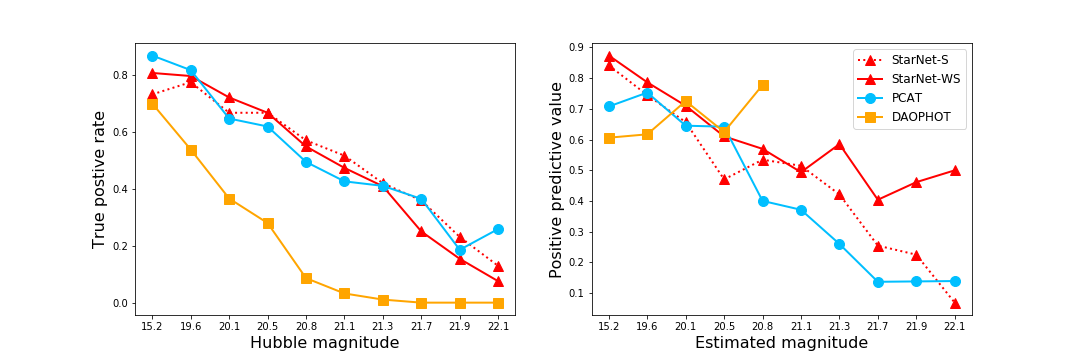
\includegraphics[width=0.99\textwidth]{figures/summary_statistics_m2.png}
    \caption{True positive rate and positive predicted value of various cataloging
    procedures on M2, plotted against magnitude percentile.
    Smaller magnitudes correspond to brighter stars. }
    \label{fig:summary_stats}
\end{figure}

In figure~\ref{fig:example_subimages}, we display four $10\times10$ subimages, and plot
our MAP catalog against the Hubble catalog. We also display the DAOPHOT catalog and one catalog sample from PCAT.

\begin{figure}[h]
    \centering
    \vspace{-3cm}
    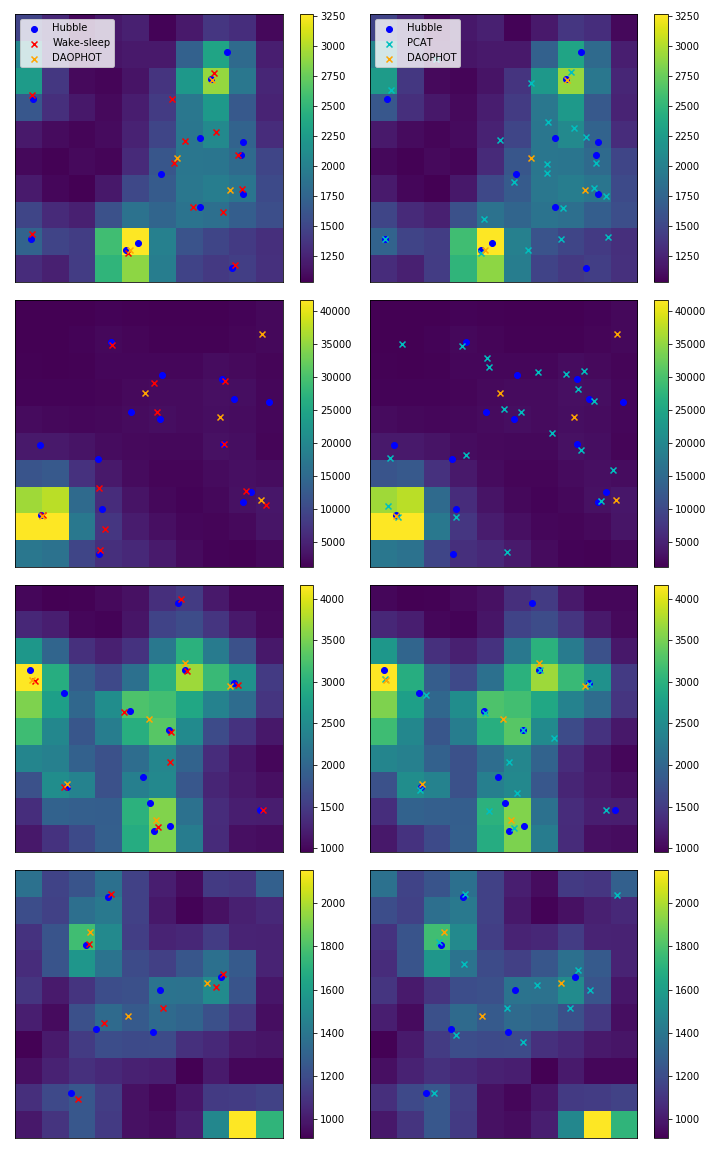
\includegraphics[width=0.8\textwidth]{figures/example_subimages.png}
    \vspace{-3cm}
    \caption{Estimated catalogs on four 10$\times$10 subimages from
    M2. Blue dots are Hubble stars brighter than the 22nd magnitude.
    Starnet, Portillos, and DAOPHOT estimated stars are in
    red, cyan, and orange x's, respectively. }
    \label{fig:example_subimages}
\end{figure}


In figure~\ref{fig:example_subimages_sampled}, we display the sampled catalogs from both our 
wake-sleep trained approximate posterior as well as from PCAT. Assuming the MCMC
of PCAT converged to the true posterior, we see that our uncertainty estimates
were generally larger. This is expected from the discussion of section~\ref{sec:kl_q_p}. 

\begin{figure}[h]
    \centering
    \vspace{-3cm}
    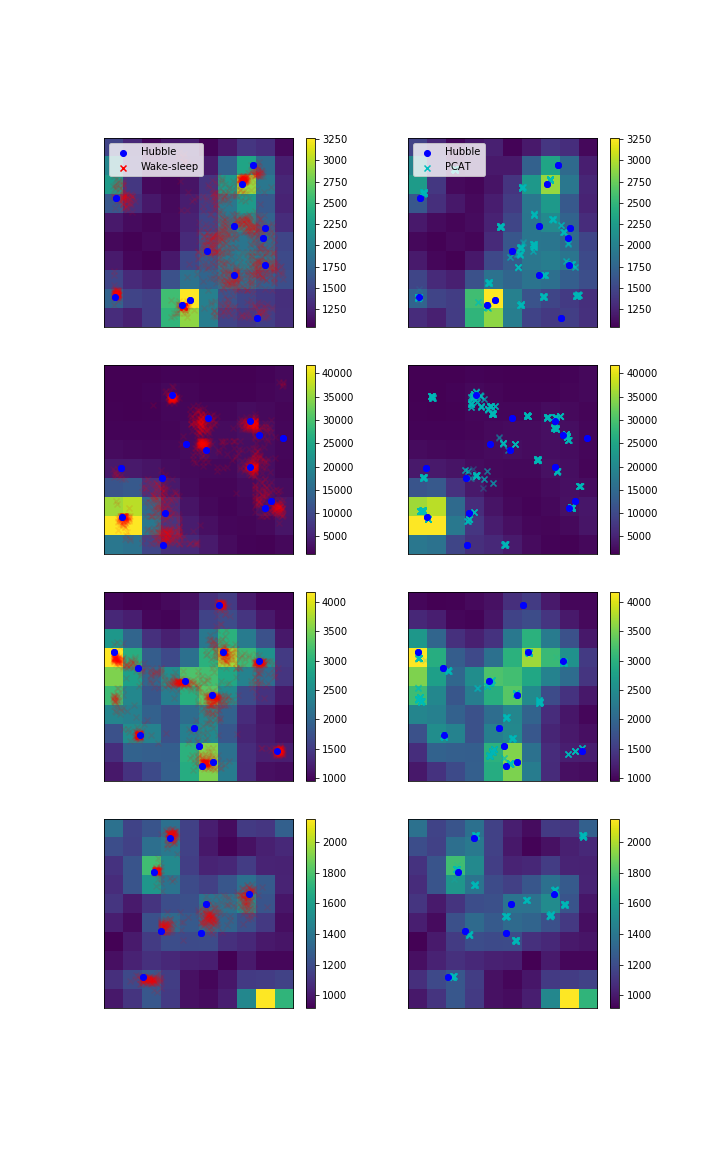
\includegraphics[width=0.8\textwidth]{figures/example_subimages_samples.png}
    \vspace{-3cm}
    \caption{Four 10$\times$10 subimages from
    M2. Blue dots are Hubble stars brighter than the 22nd magnitude.
    We print display the posterior samples from our variational
    posterior (left) and from the MCMC chain of Portillos (right). }
    \label{fig:example_subimages_sampled}
\end{figure}

In figure~\ref{fig:z-score_calibration} we examine the calibration of our uncertainties. We evaluated our approximate posterior obtained from wake-sleep training, conditioning on the true number of stars in the Hubble catalog. Thus, each star in our estimated 
catalog was matched with exactly one Hubble star (we found the permutation of the Hubble stars that had the largest log-likelihood under our variational distribution $q_\eta$). For each star, we computed the z-score $(y - \hat y) / \hat \sigma$, where $y$ is the true log-flux or 
logit-location; $\hat y$ is the mean of the Gaussian variational distribution, and $\hat\sigma$  its standard deviation. If the uncertainties were perfectly calibrated, the distribution of the 
z-scores would be a standard Gaussian. We found the empirical variance of the z-scores
to be approximately one (TODO: report values). There was a slight upward downward bias in our estimated fluxes, suggesting some degree of model mis-specification. 

\begin{figure}[h]
    \centering
    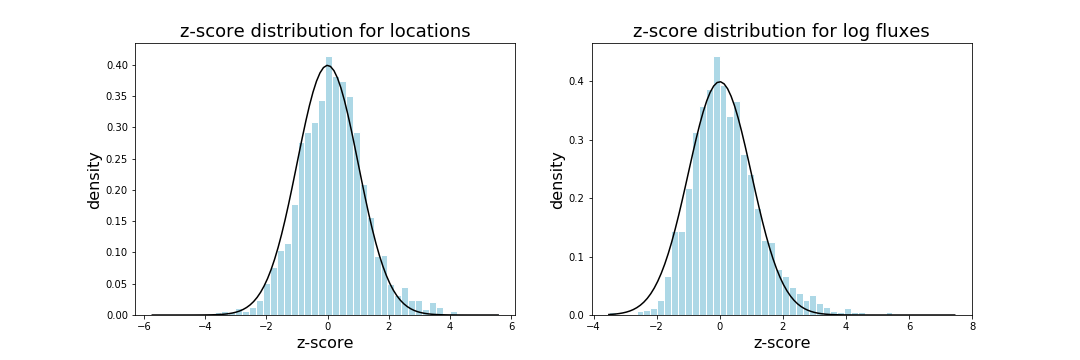
\includegraphics[width=0.99\textwidth]{figures/z-score_calibration.png}
    \caption{The calibration of uncertainties in our variational posterior. Conditional on the true number of stars, we computed the z-score of the true logit-location or log-flux evaluated at our
    variational posterior. }
    \label{fig:z-score_calibration}
\end{figure}

We plot the distribution of estimated r-band fluxes in figure~\ref{fig:luminosity_fun_m2}. We compared 
against the distribution of F606W-band fluxes in the HST catalog. While the Hubble F606W-band has a broader absorption range than the SDSS r-band, they are centered at roughly the same wavelength. For PCAT, we display the flux distribution from single catalog sample; for our variational 
posterior, we use our MAP catalog. We see that DAOPHOT returned fluxes only up to $\approx21$ mag; 
conversely, PCAT greatly over-estimated the number of dim stars with magnitude less than 21 mag. Our flux distribution came closest to the distribution of the HST catalog. 

\begin{figure}[h]
    \centering
    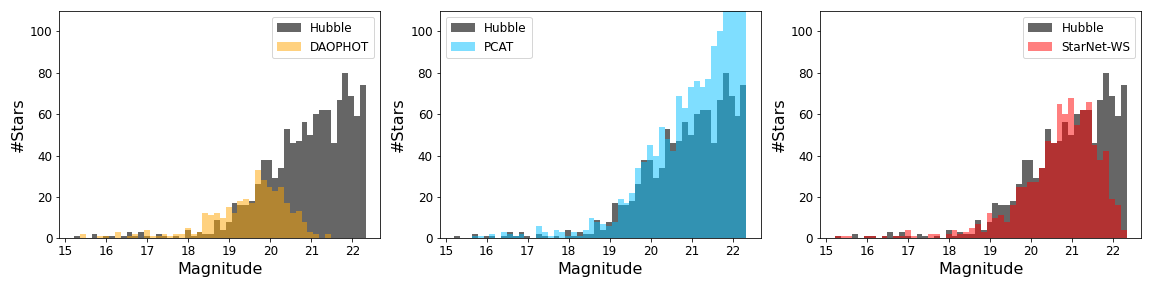
\includegraphics[width=0.99\textwidth]{figures/luminosity_fun.png}
    \caption{Source magnitude histograms on M2. }
    \label{fig:luminosity_fun_m2}
\end{figure}

Finally, we print the estimated color-magnitude diagrams in figure~\ref{fig:cmd_m2}. While the Hubble F606W-band corresponds roughly to the SDSS $r$-band, there is no such correspondence for the SDSS $i$-band. Thus, using the Hubble locations, we estimated the ``true" i-band fluxes using maximum 
likelihood (using the likelihood defined in section~\ref{sec:gen_model}). We used this estimated $i$-band flux and the Hubble F606W-band flux to define the ``true" color. We again compared with the catalog returned by DAOPHOT, PCAT, and wake-sleep. We see that DAOPHOT did not capture the full spectrum of colors; of all three methods, PCAT seemed to best capture the color spectrum. All three methods however, were able to capture the arm thing (TODO there is a name for this ... main sequence turnoff?) that branches off at low magnitudes. 

\begin{figure}[h]
    \centering
    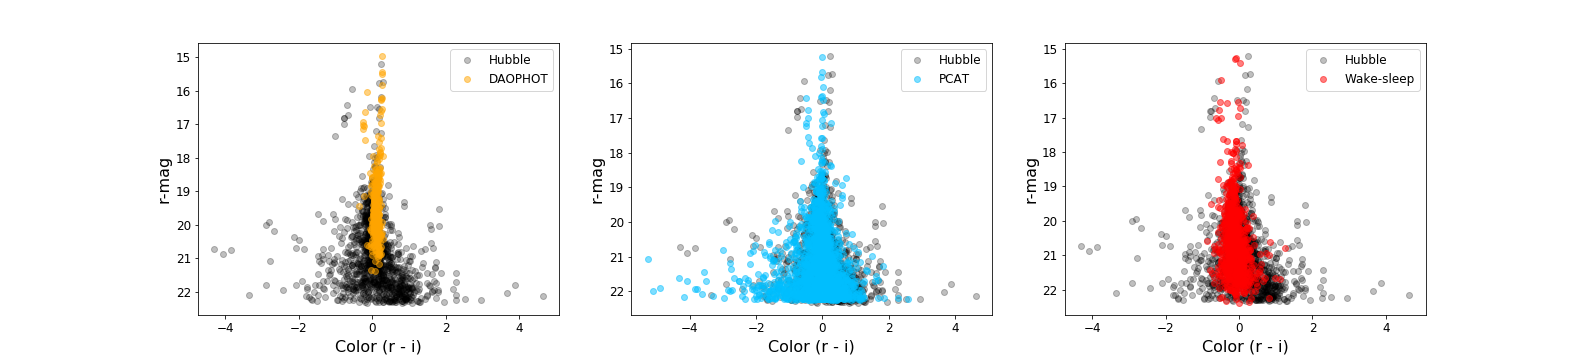
\includegraphics[width=0.99\textwidth]{figures/cmd.png}
    \caption{Color magnitude diagrams on M2. }
    \label{fig:cmd_m2}
\end{figure}


\subsection{Estimation of model parameters}
In this section, we examine our estimated model parameters. As shown in the previous section, wake-sleep improved the catalog over sleep-only. In table~\ref{tab:chi-square-stats1}, we
print the negative log-likelihood $- \log \Prob_\phi(X | N_{H}, \ell_{H}, f_{H})$ for various model parameters $\phi$, where $N_{H}, \ell_{H}, f_{H}$ are the ground truth
values from the Hubble catalog (though the $i$-band flux needs to be estimated, as above). 

We compared the log-likelihood under the default SDSS estimates of the background and the PSF with the estimates found using wake-sleep, and found that wake-sleep improved the log-likelihood. We also compared against the ``Hubble estimate" of the background and PSF, obtained by minimizing 
$- \log \Prob_\phi(X | N_{H}, \ell_{H}, f_{H})$ for $\phi$ directly. 

This table suggests that the largest source of model misfit is the background. A significant decrease occurred by switching from the SDSS background to the Hubble-estimated background. 
But even using the Hubble-estimated background, switching from the SDSS PSF to our wake-sleep PSF still improved the log-likelihood. 

\input{tables/chi_sq_stats.txt}

As evidenced in figure~\ref{fig:psf_profiles}, our wake-sleep PSF did not change the SDSS PSF significantly. The greatest change was in the r-band PSF, where the SDSS PSF was most different from the Hubble-estimated PSF. 

\begin{figure}[h]
    \centering
    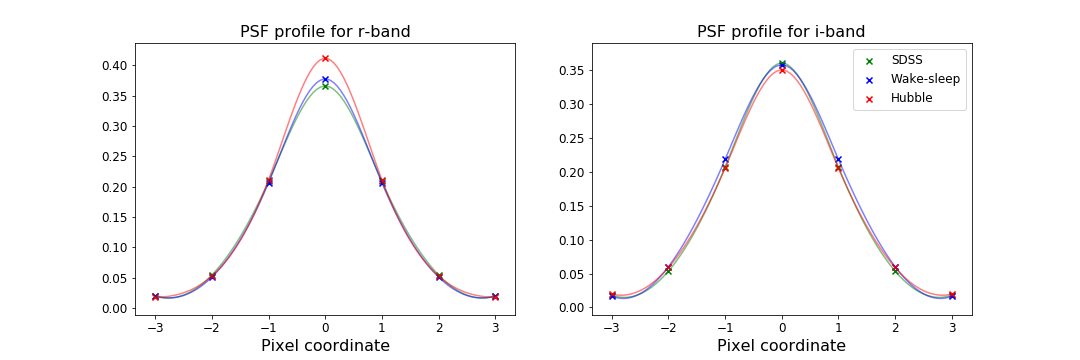
\includegraphics[width=0.99\textwidth]{figures/psf_profiles.png}
    \caption{Estimated versus true PSF profiles on M2. The Hubble PSF was
    obtained by optimizing the likelihood conditioned on locations and fluxes
    from the Hubble catalog. }
    \label{fig:psf_profiles}
\end{figure}


% \multicolumn{1}{p{5cm}}{\raggedleft Chi sq. \\ (with Hubble back.)}
% \caption{
% Chi-squared statistics for SDSS, wake-sleep, and Hubble estimated model parameters.
% The chi-squared statistic is defined as
% $\sum_{bij}\frac{([\text{obs.image}]_{bij} - [\text{recon.image}]_{bij})^2}{[\text{recon.image}]_{bij}}$.
% In the middle column, ``model parameters" refer to both background and PSF.
% In the right column, we fix the background to the Hubble estimate, and examine
% chi-squared statistics as the PSF varies.}

\subsection{Sparse field test}
As discussed in section~\ref{sec:runtime}, our approach has the potential 
to scale up to large astronomical surveys. We chose the image of M2 to 
test our method because ``ground truth" could be obtained from Hubble images 
to validate our results. However, most regions of the sky are much less 
crowded than M2. 

We applied our method to SDSS run 94, camcol 1, and field  12, 
a region of the sky with star density more typical of the SDSS survey. 
After 10 minutes of training, we produced a catalog on the full $1489\times 2048$ image in $\approx2$ seconds. 

We chose this SDSS image because it is contained in Stripe 82, a region of the sky repeated imaged by SDSS. Averaging images from different runs boosts the signal to noise ratio and this {\itshape co-added} image can be analyzed to obtain a ground truth. 

Because this region of the sky contains galaxies, we trained only the sleep-phase (otherwise the model will try to explain both stars and galaxies in the wake-phase). 
A future paper will extend our generative model to include galaxies. In 
figure~\ref{fig:sparse_field}, we plot a $500\times 500$ subimage with 
our MAP catalog overlayed with the ground truth. We also report the 
TPR, comparing the stars in the co-added image with our estimated stars. (We have extraneous defections that are due to galaxies and thus 
do not report the PPV). Of the stars in the co-added catalog with brightness at least $22.5$mag, we achieved a TPR of 90\%. 


\begin{figure}
    \centering
    \begin{subfigure}[!t]{0.45\textwidth}
        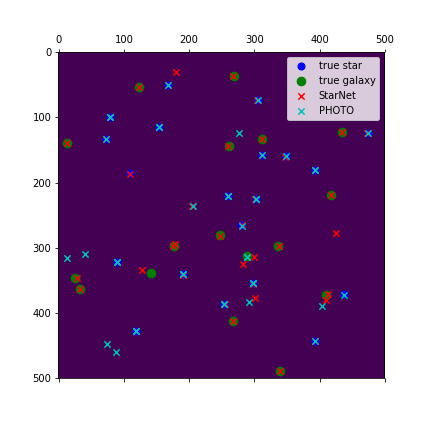
\includegraphics[width=\textwidth]{figures/sparse_field_detections.png}
        \label{fig:sparse_field_detect}
    \end{subfigure}
    \begin{subfigure}[!t]{0.54\textwidth}
        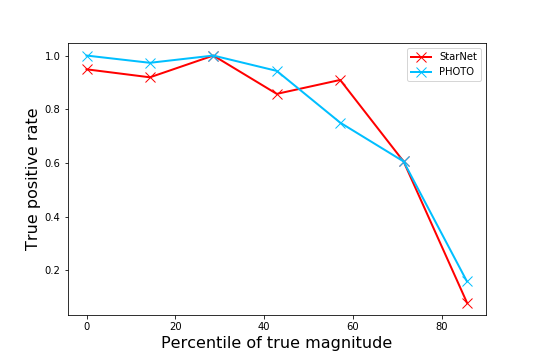
\includegraphics[width=\textwidth]{figures/sparse_field_tpr.png}
        \label{fig:sparse_field_tpr}
    \end{subfigure}
    \caption{sparse field}
    \label{fig:sparse_field}
\end{figure}
